% !TEX encoding = UTF-8 Unicode
\documentclass[a4paper]{article}

\usepackage{multicol}
\usepackage{color}
\usepackage{url}
\usepackage[T2A]{fontenc} % enable Cyrillic fonts
\usepackage[utf8]{inputenc} % make weird characters work
\usepackage{graphicx}

\usepackage[english,serbian]{babel}
%\usepackage[english,serbianc]{babel} %ukljuciti babel sa ovim opcijama, umesto gornjim, ukoliko se koristi cirilica
\usepackage[unicode]{hyperref}
\hypersetup{colorlinks,citecolor=green,filecolor=green,linkcolor=blue,urlcolor=blue}

\usepackage{listings}

%\newtheorem{primer}{Пример}[section] %ćirilični primer
\newtheorem{primer}{Primer}[section]

\definecolor{mygreen}{rgb}{0,0.6,0}
\definecolor{mygray}{rgb}{0.5,0.5,0.5}
\definecolor{mymauve}{rgb}{0.58,0,0.82}

\lstset{ 
	backgroundcolor=\color{white},   % choose the background color; you must add \usepackage{color} or \usepackage{xcolor}; should come as last argument
	basicstyle=\scriptsize\ttfamily,        % the size of the fonts that are used for the code
	breakatwhitespace=false,         % sets if automatic breaks should only happen at whitespace
	breaklines=true,                 % sets automatic line breaking
	captionpos=b,                    % sets the caption-position to bottom
	commentstyle=\color{mygreen},    % comment style
	deletekeywords={...},            % if you want to delete keywords from the given language
	escapeinside={\%*}{*)},          % if you want to add LaTeX within your code
	extendedchars=true,              % lets you use non-ASCII characters; for 8-bits encodings only, does not work with UTF-8
	firstnumber=1000,                % start line enumeration with line 1000
	frame=single,	                   % adds a frame around the code
	keepspaces=true,                 % keeps spaces in text, useful for keeping indentation of code (possibly needs columns=flexible)
	keywordstyle=\color{blue},       % keyword style
	language=Python,                 % the language of the code
	morekeywords={*,...},            % if you want to add more keywords to the set
	numbers=left,                    % where to put the line-numbers; possible values are (none, left, right)
	numbersep=5pt,                   % how far the line-numbers are from the code
	numberstyle=\tiny\color{mygray}, % the style that is used for the line-numbers
	rulecolor=\color{black},         % if not set, the frame-color may be changed on line-breaks within not-black text (e.g. comments (green here))
	showspaces=false,                % show spaces everywhere adding particular underscores; it overrides 'showstringspaces'
	showstringspaces=false,          % underline spaces within strings only
	showtabs=false,                  % show tabs within strings adding particular underscores
	stepnumber=2,                    % the step between two line-numbers. If it's 1, each line will be numbered
	stringstyle=\color{mymauve},     % string literal style
	tabsize=2,	                   % sets default tabsize to 2 spaces
	title=\lstname                   % show the filename of files included with \lstinputlisting; also try caption instead of title
}


\begin{document}
	
	\title{Komunikacija preko mreže\\ \small{Seminarski rad u okviru kursa\\Metodologija stručnog i naučnog rada\\ Matematički fakultet}}
	
	\author{Bakić Katarina, Milovanović Nenad, \\Kovačević Matija, Kovačević Nikola\\
	ina.bakic95@gmail.com, nenadmilovanovic6@gmail.com, \\kovacevmatija@gmail.com, nik\_ko\_@outlook.com}
	
	\date{28. april 2019.}
	
\maketitle
\abstract{
U ovom radu smo pokušali da Vam prikažemo deo teme komunikacije preko mreže. U početku smo obradili temu  izgubljenog poverenja na Internetu, da nije sve što nađemo i pročitamo na Internetu sigurno i verodostojno. Naveli smo određene primere prevare i zloupotrebe u cilju da korisnici što više obrate pažnju i sačuvaju svoj identitet. Svesni smo činjenice da je komuniciranje preko mreže sve više zastupljeno, pa se samim tim pored prevara javlja i zavisnost. Naveli smo određene uslove zavisnosti i statistike rasprostranjenosti. Za kraj, rad upotpunjujemo pričom o zavisnosti od društvenih mreža i Internet igara, kao i prikazom posledica (psihičkih i fizičkih). Ova tema je veoma rasprostranjena i aktuelna, pa se nadamo da smo uspeli u našem cilju da Vam ukažemo na velike probleme i moguća rešenja.}
	
\tableofcontents

\newpage

\section{Uvod}
\label{sec:uvod}
 Internet je globalna mreža koja nam daje mogućnost komunikacije i deljenja resursa na Zemlji. Mrežne komunikacije imaju poseban značaj, sve oko nas se pretvara u kompjuter \cite{dataAndGoliath}. Njihovim razvojem je omogućeno poslovanje među firmama, pristup određenim nedostižnim informacijama, prodaja, kupovina, komunikacija sa prijateljima putem društvenih mreža. Komunikacija se ne odvija samo putem telefona i računara, zastupljena je i u auto industiriji, medicini... Ovaj vid komunikacije nam omogućava da u svakom trenutku pronađemo ono što nam je potrebno od podataka.\newline
 Koliko god prednosti da ima, toliko ima i mana. Kako se Internet razvija i postaje dostupan sve većem broju ljudi, tako i broj zavisnika i prevara raste. Ljudi sve više vremena provode za računarima, pametnim telefonima i sličnim uređajima, a deca sve manje izlaze na igrališta sa svojim vršnjacima. Javlja se velika zavisnost od Interneta (globalni problem) i zdravstveni problemi (na primer, problem sa vidom). Računari i računarske mreže se danas mogu zloupotrebljavati na razne načine. Lažni podaci i profili, krađa i zloupotreba tuđeg identiteta putem mreže su samo neki od problema sa kojima se možemo sresti svakodnevno na Internetu.\newline
 Počeli smo pričom o izgubljenom poverenju (poglavlje \ref{sec:izgubljeno_poverenje}), kako bismo istakli moguće probleme i njihove posledice. Pokušali smo da Vam prikažemo problem verodostojnosti podataka u okviru dela \ref{subsec:podnaslovIP1} i da Vam skrenemo pažnju na neke vrste Internet prevare u odeljku \ref{subsec:podnaslovIP2}. Kako su posmatranje i kontrola na Internetu sve češće, kroz određene primere želimo da Vas upoznamo u delu \ref{subsec:podnaslovIP4}. Nakon toga priču širimo na opštepoznati problem, problem zavisnosti. Kako je možete prepoznati (koji su njeni kriterijumi) i koliko je rasprostranjena možete da pogledate u poglavlju \ref{subsec:podnaslovZI1}. Pomoću primera zavisnosti od društveniih mreža (deo \ref{subsec:podnaslovIP5}) i Internet igara (odeljak \ref{subsec:podnaslovIP6}) treba da shvatimo kako ovaj problem nije jedinostavan. On ostavlja određene posledice, koje možete pročitati u poglavlju \ref{subsec:podnaslovZI2}.
\section{Izgubljeno poverenje}
\label{sec:izgubljeno_poverenje}
Poverenje je jedna od  bitnijih stavki u odnosu dve ili više osoba. Informacije koje dospeju na Internet su veoma nepouzdane i sklone su promenama.

\subsection{Vikipedija}
\label{subsec:podnaslovIP1}

Vikipediju (eng. Wikipedia) doživljavamo kao veliki i bogat skup informacija. Ona predstavlja jedan od najposećenijih sajtova na svetu. Na željenu temu možemo da dobijemo po nekoliko desetina ili stotina članaka. Ipak, na Vikipediji nije moguće razlikovati istinite i lažne informacije, ukoliko ne pronađemo adekvatne knjige i verodostojne podatke na nekom sigurnijem mestu. Javno je dostupna i svako joj može pristupiti, moguće je da više autora napiše jedan članak. Izvor tih informacija može da ostane potpuno nepoznat. Sve te informacije koje se postave mogu povremeno da se menjaju, pa samim tim one prolaze kroz više izvora. Na samim korisnicima je da procene verodostojnost ponuđenih informacija, ukoliko su odlučni da ih koriste. \\Deca u školama najčešće koriste ove izvore prilikom izrade svojih domaćih zadataka, prezentacija i slično. Oni u tom periodu o verodostojnosti tih podataka ne razmišljaju. Mnogima su informacije sa Vikipedije bile kvalitetne i proverene, ali postoje i one koje nisu ni blizu istinitosnih.
\begin{primer}
Korsgaard i Jensen su 2009. godine predložili određene promene na softveru za Vikipediju, kako bi ocene koje su prethodno bile na člancima bile ubačene i u poslednje verzije. Na taj način bi se prikazalo da je problem verodostojnosti bar malo rešen ukoliko u novijoj verziji ima bolju ocenu. „WikiTrust", na primer boji pozadinu svake reči u skladu sa kredibilitetom, na osnovu toga koliko je puta reč preživela uređenje članka \cite{tInOnl}.
\end{primer}

\subsection{Internet prevare}
\label{subsec:podnaslovIP2}
Ljudi se oslanjaju na komunikaciju putem Interneta, Internet bankarstvo i Internet trgovinu. Veoma je bitno da korisnici budu zaštićeni i da sačuvaju svoje privatne informacije, kako ne bi došli do neželjene situacije. Videćemo određene vrste Internet prevare:
\begin{itemize}
\item\textbf{Pecanje} (eng. phishing) predstavlja dobro poznatu vrstu napada socijalnog inženjeringa. Osnovni cilj je krađa identiteta korisnika, odnosno uzimanje njegovih ličnih podataka i želja da se nanese šteta firmama. Najčešće se napadi organizuju preko elektronskih poruka i stranica, koje izgledaju skoro isto kao originalne (verodostojne Internet stranice i poruke određenih firmi, klijenata...). Prilikom nepažnje korisnika, koji su meta napada, ostavljaju se lični podaci, kao sto su: privatni broj telefona, broj računa u banci, kućna adresa ili se čak omogućava pristup računarima i telefonima. U želji da se korisnik što više uveri da se radi o pravim stranicama nude mu se poprilične svote novca, posao, putovanja...\\Ovaj vid prevare se povećava pojavom i naglim razvojem mobilnih uređaja. Kako su ekrani manji, korisnici teže mogu da primete da se radi o prevari. Korisnici se u ovo vreme ne razdvajaju od svojih telefona, provode previše vremena pri korišćenju istog, pa samim tim je mnogo lakše da budu meta napada. Prilikom krađe bankovnih računa, oni koji napadaju se pretvaraju da su normalni korisnici, ponašaju se onako kako se dati korisnik i pre toga ponašao, kako se ne bi previše brzo primetila razlika i otkrila krađa. 
\\Na primer, korisnik može da dobije poruku za određen bankovni promet, koja zahteva korisničko ime i šifru. Ukoliko ne primeti nikakvu razliku u odnosu na verodostojnu bankovnu transakciju, dešava se da njegov bankovni račun bude ispražnjen. Takođe napadač veoma lako može da napravi nalog za elektronsku poštu (sličan nazivu određene kompanije), pa da po hitnom postupku traži od kupca prenos novca na novi račun. \\U ovakvim situacijama bi bilo poželjno proveriti sa stvarnim kompanijama o čemu se radi, inače je prevara zasigurana. Ukoliko ne očekujemo određeni poziv ili elektronsku poštu bolje da se ne upuštamo u to. Naredna slika \ref{fig:phishing} predstavlja primer pecanja putem elektronske pošte.
\end{itemize}
\begin{figure}[h!]
\begin{center}
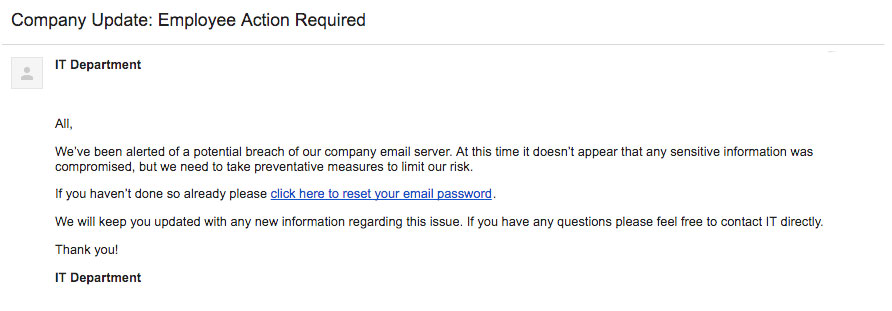
\includegraphics[scale=0.4]{msnr_phishing.jpg}
\end{center}
\caption{Primer pecanja }
\label{fig:phishing}
\end{figure}

\begin{primer}
Na Amazonu skoro svi imaju račune, pa je preko njega veoma lako doći do poverenja i naivnosti klijenata. Korisnik može da zanemari malu izmenu ukoliko je napad veoma dobro organizovan, pa ukoliko je ‘o’ zamenjeno sa ‘0’ ili nekom približnom oznakom, on to neće tako lako primetiti \cite{6exp}.
\end{primer}

Dobar način da se ovaj vid prevare izbegne pri pretraživanju Interneta je obeležavanje url stranica koje su nam bitne i pouzdane. Prevare ovakvog tipa su sve češće i lako se može postati njihova žrtva.

\begin{itemize}
\item \textbf{„Nigerijska prevara”} nastaje oko 1980. godine u Nigeriji. Ona predstavlja vrstu prevare kod koje se od žrtve traži pomoć za transfer novca. Prevarant na primer objašnjava da mu je novac zarobljen u inostranstvu i da mu je potrebna pomoć oko transfera, kako bi uspeo da se oslobodi poreza. On za tu uslogu nudi veliku količinu novca (od 10\% do 30\% u odnosu na celokupan iznos), a žrtva na taj način postaje njegov saučesnik u zločinu. Od žrtve se zahteva da pošalje svoje detalje bankovnog računa ili da otvori račun u određenoj banci, kako bi na taj način mogli da pristupe njegovim podacima. Ovaj vid prevare se obično odvija putem elektronske pošte. 
\begin{primer}
Na teritoriji Republike Srbije u toku 2008. i 2009. godine od strane oštećenih lica prijavljeno je devet krivičnih dela prevare sa elementima „Nigerijskih prevara“ \cite{nig}.
\end{primer}

\end{itemize}
\begin{itemize}
\item\textbf{Društvene mreže} su jedna od najpopularnijih oblasti istraživanja i razvijanja. Ljudi zahvaljujući njima menjaju način razmišljanja i imaju drugačiji pogled na sve oko sebe. Neke od popularnijih mreža su Fejsbuk (eng. Facebook), Skajp (eng. Skype), Tviter (eng. Twitter), Instagram i skoro svi imaju nalog na bar jednoj mreži. Sve što korisnici postavljaju i šalju na društvenim mrežama predstavlja njihov prikaz ličnosti. Njihov cilj je međusobno druženje i komunikacija sa prijateljima, koje ne možemo svakodnevno da vidimo. Ipak, na njima ima dosta krađa identiteta, napada na pojedince, svađa, pornografije i sličnih loših stvari.\\Dešava se da pojedini roditelji tek rođenoj deci otvaraju profile na nekoj od društvenih mreža, pa samim tim ih dovode u veliku opasnost postavljajući javno njihove slike, a da ne slute da te slike mogu biti zloupotrebljene. Na ovim mrežama se javlja veliki broj lažnih profila.
Napadači obično koriste te lažne profile sa velikom pažnjom, kako bi povećali nivo poverenja. Oni koji prave profile sa tuđim identitetom ili hakuju željene profile, obično veoma dobro poznaju tu osobu \cite{fakePr}. Svi ti lažni profili mogu biti veoma opasni ako se ne otkriju na vreme, pa oni predstavljaju sve veće probleme.
\end{itemize}
\subsection{Masovna kontrola, posmatranje i privatnost na Internetu}
\label{subsec:podnaslovIP4}
\indent\indent Prosečni korisnici Interneta uglavnom nisu ni svesni da za korišćenje najpopularnjih „besplatnih” veb servisa (pretraživači, e-mail, društvene mreže..) zauzvrat odaju ogroman broj podataka i informacija o sebi. Zbog neinformisanosti imaju lažan osećaj sigurnosti i neosnovano poverenje da im je omogućena anonimnost. Većina tih servisa se, bez znanja korisnika, bavi masovnim skladištenjem podataka i njihovom analizom (eng.~{\em data mining}). Rezultate dobijene iz analize podataka mogu koristiti za manipulaciju na raznim sektorima, poput ekonomskog tržista, političkih ciljeva, marketinga i slično. Pored obrade podataka društvenih masa, bez ikakvih ograničenja se mogu izdvojiti podaci i o pojedincima.\newline Počinioci ovakvih radnji se uglavnom mogu svrstati u dve određene grupe, privatne korporacije i državne agencije. Motiv u slučaju privatnih korporacija je naravno profit. Dobro poznavanje tržista i korisnika njihovih proizvoda kao posledicu daje visok profit. Motiv kod državnih agencija je, naivno gledano, sigurnost države i njenih stanovnika (npr. sprečavanje terorizma), iako je često veći akcenat na kontroli i smanjenju privatnosti sopstvenih građana. Dalje ćemo kroz nekoliko najzanimljivijih primera koji su izloženi javnosti pokazati kako servise na Internetu treba koristiti sa velikom dozom nepoverenja.\\\textbf{Uzbunjivač (eng.~{\em whistleblower})} - \textit{naziv za hrabrog pojedinca koji iz moralnih razloga odlučuje da uz sopstveni rizik progovori o nezakonitim i neetičkim radnjama svojih nadređenih.}

\begin{primer}
Edward Snowden, jedan od najpoznatijih uzbunjivača otkriva mnoge operacije državnih organizacija SAD koje narušavaju privatnost velikog dela korisnika Interneta. U dokumentima koje objavljuje pokazuje kolaboraciju mnogih država („Five Eyes” , alijansa koja se sastoji od Australije, Kanade, Novog Zelanda, Britanije i SAD-a) u projektima koji su korišćeni za globalno posmatranje i otkrivanje privatnih podataka na mreži \cite{noPlaceToHide}. Neki od značajnijih programa su koje je Edward izneo javnosti su:
\begin{itemize}
\item \textbf{MUSCULAR} je softver koji presreće mnoštvo podataka pristupom kablovima ispod površine mora, kao i nelegalnim pristuom data centrima uglavnom korporacija Yahoo i Google \cite{noPlaceToHide}.
\item \textbf{PRISM}, softver pod okriljem američke Nacionalne Sigurnosne Agencije (NSA), je pored velikih korporacija kao izvora privatnih podataka (Microsoft, Facebook, Google, Apple...) presretao i podatke u toku prenošenja na kičmenom stubu (engl.~{\em backbone}) Interneta \cite{noPlaceToHide}.
\item \textbf{XKEYSCORE}, program za opšti pristup bilo kakvim informacijama koje prolaze kroz Internet, jednostavnim upitom i pretragom pokazuje bilo čije e-mailove, privatne poruke, telefonske pozive, fajlove, lokacije i ostale razne informacije. Procena je da Xkeyscore dnevno prikupi oko 1.7 milijardu poruka, poziva i drugih podataka \cite{noPlaceToHide}.
\item \textbf{BULLRUN} je softver koji služi za razbijanje enkriptovanih poruka na mreži \cite{noPlaceToHide}.
\end{itemize}
\end{primer}

\begin{primer}
Makmilijan Šrems, tadašnji dvadeset trogodišnji student prava u
Austriji, je 2011. godine od Facebook-a tražio sve privatne podatke koje su sakupili o njemu. Pored zahteva za podatke je i tužio Facebook jer su nelegalno prosleđivali privatne podatke korisnika društvene mreže projektu PRISM\cite{noPlaceToHide} za koji je zadužena NSA. Nakon dvogodišnje sudske parnice, Maks dobija od Facebook-a pdf fajl koji sadrži isključivo njegove lične podatke i koji ima čak 1200 stranica \cite{marxSchremsFT}.
\end{primer}

\begin{primer}
Januara 2012. godine, Facebook pravi psihološki eksperiment koji traje jednu nedelju. U eksperimentu učestvuje 689,003 profila koji su izloženi emotivnoj manipulaciji. Ovim se tragalo za odgovorom da li se emotivna zaraza može širiti kroz mrežu. Zapravo, Facebook je podelio učesnike testa na određene grupe, gde je svaka grupa dobijala isključivo objave koje izazivaju ili pozitivne ili negativne emocije na početnoj strani društvene mreže. To je rezultovalo u prenošenju emocija, gde je grupa koja je viđala samo pozitivne objave pokazala uvećane srećne emocije i analogno 	za grupu koja je izložena negativnim emocijama \cite{facebookExperiment}.
\begin{quotation}
\textit{„We show, via a massive (N = 689,003) experiment on Facebook, that emotional states can be transferred to others via emotional contagion, leading people to experience the same emotions without their awareness.
"Data from a large real-world social network, collected over a 20-y period suggests that longer-lasting moods (e.g., depression, happiness) can be transferred through networks.”}
\begin{flushright}
-\em{Deo zaključka iz originalnog naučnog rada \cite{facebookExperiment}.}
\end{flushright}
\end{quotation}
\end{primer}

\begin{primer}
Sredinom 2009. godine, Amazon izaziva veoma ironičnu situaciju. Nakon nekoliko hiljada prodatih e-book kopija knjige "1984" Džordža Orvela, ispostavlja se da izdavačka kuća tih kopija nema autorska prava. Amazon čitav problem rešava tako što bez znanja korisnika briše sve kopije na njihovim uređajima Kindle. Ovaj postupak je opisan kao „Orwellian” i potegao je mnoga pitanja o tome kolika prava Amazon ima \cite{dataAndGoliath}.
\\\textbf{„Orwellian”} - \textit{pridev koji opisuje nedostatak slobode i prava, propaganda, posmatranje, diktaturu...}\\
\end{primer}

\begin{primer}
Jednostavna Android aplikacija „Brightest Flashlight 
Free” je pored svoje jedine funkcije, paljenja i gašenja blic LED svetla, nelegalno skupljala podatke u vidu lokacija korisnika. Aplikacija je imala izmedju 50 i 100 miliona korisnika i podaci o njihovim lokacijama su kupovale korporacije za marketing i reklame \cite{dataAndGoliath}\cite{flashlightApp}.\\
\end{primer}

\begin{primer}
Mobilni telefoni su u stanju da svakog trenutka pokazuju lokaciju na kojoj se nalaze. Čak je i rađeno istraživanje gde su praćena kretanja određenog broja ispitanika preko moblinog telefona. Na osnovu skupljenih podataka o njihovim kretanjima, istraživači su uspeli sa iznenađujućom tačnošću da predvide njihove trase kretanja za naredna 24 sata. Za vreme revolucije u Kijevu, 2014. godine, veliki broj učesnika protesta je dobilo SMS poruku upozorenja da učestvuju u demonstracijama. Poruku su dobile jedino osobe koje su bile u centru protesta, na osnovu lokacija koje su odašiljali njihovi telefoni \cite{dataAndGoliath}.
\end{primer}

	Vredni spomena su još neizbežnost skupljanja podataka od strane Googla uz pomoć njihovih {\em kolačići trećeg lica} (eng.~{\em third-party cookie}) i \textit{Google Analytics}. Google će dolaziti do vaših informacija čak i ako ne koristite njihov pretraživač. Oni mogu da skladište oko 15 eksabajta (1 eksabajt = $10^{18}$ bajtova). Procenjuje se da je Google najaktivniji po pitanju skladištenju i korišćenju podataka korisnika. Poznata je i takozvana marketing diskriminacija. Funkcioniše tako što analizom podataka daje različite uslove i reklame korisnicima Interneta radi postizanja većeg profita. Kao primer, jedno od istraživanja pokazuje da su osobe ženskog pola više sklone kupovini kozmetičkih proizvoda ponedeljkom jer tim danom u nedelji imaju manji nivo samopouzdanja u odnosu na ostale dane. Naravno, stvari poput ovih se koriste za postavljanje reklama u pravo vreme sve radi profita, ne vodeći previše računa o etici \cite{dataAndGoliath}\cite{theNetDelusion}.

	Ovo su samo od nekih mnogobrojnih primera koji nam pokazuju da korišćenje Interneta nije toliko "besplatno" i naivno koliko se misli. Iako se trenutno ne može uraditi mnogo stvari povodom toga, poželjno je što više proširiti informisanost o tome šta se sve zapravo dešava na mreži.

\section{Zavisnost od interneta}

Razvoj interneta i mogućnosti koje on nudi dovodi do toga da ga sve više ljudi koristi u sve većoj meri.
Kao što je slučaj sa narkoticima i alkoholom, ljudi mogu razviti i zavisnost od Interneta. Prepoznavanje ove zavisnosti uglavnom nije jednostavno jer za razliku od prethodno pomenutih koje podrazumevaju fizičku zavisnost i ne donose nikakvu korist. Internet nudi dosta benefita i njegovo korišćenje je gotovo neizbežno u svakodnevnom životu. Stoga, mnogi znaci zavisnosti od Interneta kao na primer vreme provedeno koristeći Internet mogu biti opravdani. Postoje podeljena mišljenja oko toga da li zavisnost od Interneta uopšte postoji. Tradicionalno, zavisnost se definise kao kontinuirana i nekontrolisana upotreba neke hemijske supstance uprkos znanju o njenim štetnim posledicama, dok proširena definicija uključuje svako  kontinuirano i nekontrolisano ponašanje koje zavisnik prepoznaje kao štetno. Prema proširenoj definiciji ljudi mogu biti zavisni od hrane, seksa, treniranja, kockanja, korišćenja računara i drugih aktivnosti \cite{ethics}.

\subsection{Prepoznavanje i rasprostranjenost}
\label{subsec:podnaslovZI1}

Dr Kimberly Young predstavila je jedan od prvih testova za dijagozu zavisnosti od Interneta, koji je modifikacija metode za prepoznavanje zavisnosti od kockanja. Test se sastoji od 8 pitanja i ispitanik koji odgovori pozitivno na 5 ili više pitanja smatra se zavisnim \cite{ethics}.
Još jedan opšte prihvaćen metod predložio je Keith Beard u svom radu iz 2005. godine \cite{diagnostic}. Prema njemu, osoba je zavisna od Interneta ako ispunjava sledećih 5 kriterijuma:
\begin{itemize}
  \item Konstantno razmišlja o korišćenju Interneta
  \item Ostaje na mreži duže nego što je planirala
  \item Bezuspešno je pokušala da kontroliše ili prekine upotrebu Interneta
  \item Ima potrebu da provodi mnogo vremena na Internetu kako bi osetila zadovoljstvo
  \item Depresija ili razdražljivost pri pokušaju da kontroliše upotrebu Interneta
\end{itemize}

Dodatno, bar jedno od sledećih tvrđenja mora biti tačno kako bi se postavila dijagnoza:
\begin{itemize}
  \item Laganje drugih ljudi o korišćenju Interneta
  \item Koristi Internet kao način da pobegne od problema
  \item Rizikovanje gubitka bitne veze ili posla zbog Interneta
\end{itemize}

Istraživanja na temu rasprostranjenosti ove zavisnosti dolaze do različitih rezultata (od 0.3\% do čak 38\%) što je posledica korišćenja različitih metoda na različitim grupama ispitanika (npr. onlajn ispitivanja ne uzimaju u obzir ljude koji ne koriste Internet).
C. Cheng i A. Y. Li su sproveli istraživanje na ovu temu nad 89,281 ispitanikom iz 31 države \cite{prevalence}.
Prosečna starost ispitanika je 18.42 godine.
Rezultati dobijeni ovim istraživanjem prikazani su u tabeli \ref{tab:tabela1}.

\begin{table}[h!]
\begin{center}
\caption{Rasprostranjenost zavisnosti od Interneta u različitim delovima sveta.}

\begin{tabular}{|c|c|c|} \hline
Regija& Rasprostranjenost& Broj ispitanika\\ \hline
Severna Amerika &8.0\% &4,117\\ \hline
Okeanija &4.3\% &2,716\\ \hline
Severna i Zapadna Evropa &2.6\% &16,086\\ \hline
Južna i Istočna Evropa &6.1\% &27,699\\ \hline
Bliski istok &10.9\% & 3,979\\ \hline
Azija &7.1\% &34,604\\ \hline
Južna Amerika & 0.0 \% & 80\\ \hline
Ukupno &6.0\% &89,281\\ \hline 
\end{tabular}
\label{tab:tabela1}
\end{center}
\end{table}

Dobijeni rezultat pokazuje da je 6\% ljudi na svetu zavisno od Interneta. Važno je napomenuti da ispitivanje nije rađeno na području Afrike. Procena je da samo 16\% afričkog stanovništva koristi Internet(2014. godina) ali se taj broj brzo povećava. Takođe, u Južnoj Americi je bilo samo 80 ispitanika iz Kolumbije.

\subsection{Zavisnost od društvenih mreža}
\label{subsec:podnaslovIP5}

\indent\indent Kao što je već pomenuto, društvene mreže predstavljaju deo Interneta koji se najbrže razvija. U poslednjoj deceniji ovakvi sajtovi su stekli ogromnu popularnost. Prema određenim podacima, samo Facebook ima bazu od dve milijarde mesečnih korisnika dok 30\% korisnika predstavljaju osobe od 25 do 34 godine \cite{socialN}. Problem sa kojim se srećemo, pored toga što je korisnik izložen raznim rizicima u smislu sajber napada i krađe identiteta, jeste to što se pojavljuje potreba da se konstantno bude na vezi (eng. online) da bi ostao u toku sa najnovijim dešavanjima. Na ovaj način se stvara potreba za prekomernim korišćenjem društvenih mreža, pogotovo što je to, u zadnjih tri do pet godina, znatno olakšano razvojem pametnih telefona preko kojih možemo u svakom trenutku proveriti stanje na Facebook-u ili okaciti sliku na Instagram. Kod određenih korisnika, ovakva mogućnost upotrebe dovodi do simptoma koje se tradicionalno dovode u vezu sa bolestima zavisnosti prouzrokovanim hemijskim supstancama (marihuana, kokain, heroin...)  \cite{snsa}. Prekomerna upotreba društvenih mreža naročito je prisutna kod adolescenata i mladih odraslih osoba. Posledica ovoga je smanjenje socijalnih i komunikacionih veština, zbog toga što je vreme potrebno za poboljsanje istih zamenjeno vremenom na vezi zarad kratkoročne pažnje i lažnog samopouzdanja. Pojedinci su opisani kao „zajedno sami" (eng. alone together), to jest, povezani putem društvenih mreža, ali u stvari sami \cite{turkle2017alone}.
\\
\indent Na osnovu različitih istraživanja, pravljenjem veza između profila ličnosti ispitanika i njihovog vremena provedenog na društvenim mrežama, može se zaključiti da usamljenije i često depresivne osobe teže ka provođenju više vremena na društvenim mrežama, isto kao i kod zavisnika od nekih opojnih droga. Međutim, mišljenja naučnika su podeljena u stavu da li zavisnost od društvenih mreža uopšte treba klasifikovati kao poremećaj. Dok je u Kini i Južnoj Koreji zavisnost od drustvenih mreža klasifikovana kao psihički poremećaj, to nije slučaj u ostatku sveta.
\\
\begin{figure}[h!]
\begin{center}
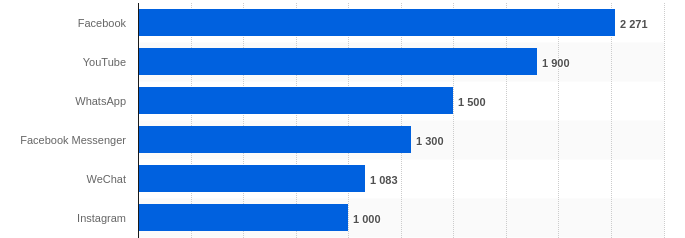
\includegraphics[scale=0.5]{top_6_networks.png}
\end{center}
\caption{Prvih šest društvenih mreža sa najviše korisnika}
\label{fig:top_networks}
\end{figure}

\subsection{Zavisnost od Internet igara}	
\label{subsec:podnaslovIP6}

%MMORPG (Masive Multiplayer Role Playing Game), Nagradne igre, Kockanje preko interneta
\indent Pre nego sto je Internet bio široko rasprostranjen, jedini način da vise ljudi zajedno igra određenu igru jeste da se sastanu na jednom mestu. Posto je razvojem Interneta omogućeno slanje i primanje velike količine podataka za par milisekundi, da biste igrali omiljenu igru sa prijateljima vise nije bilo potrebno izlaziti iz kuće. Neophodni su vam bili samo igra instalirana na kompjuteru i konekcija na Internet. Pošto je putem Interneta umrežen ceo svet, postalo je moguće da dve osobe sa dva kraja planete igraju istu igru u isto vreme. Počele su da se osnivaju Internet zajednice igraca određenih igrica (eng. Internet gaming community) i da se, između ostalog, prave takozvane MMORPG (eng. Massive Multiplayer Role Playing Game) igre, čija je glavna karakteristika da omoguće velikom broju igrača zajednički boravak u virtuelnom svetu te igre. Ovo podrazumeva pravljenje virtualnog avatara kojeg igrač pokreće. Nakon par godina postojanja ovakvog tipa igara, primećeno je da one predstavljaju idealan beg od sveta osobama nezadovoljnim svojim životom, tj. omogućavaju ljudima da žive virtuelni život od kojeg postaju zavisni. 
\\
\indent Pored MMORPG igara, jos jedan tip izrazito zavisnih igara koji se ističe je igre na sreću, odnosno klađenje. Pošto je moguće kladiti se od kuće, postaje sve vise dostupniji osobama mlađim od 18 godina, odnosno deci, kojima je zabranjen ulaz u kladionice. Međutim na ovaj način lako mogu da zaobiđu sigurnosne mere koje postoje prilikom pravljenja naloga (npr. broj godina) i da naprave porodici materijalnu štetu.

Za razliku od zavisnosti od društvenih mreža, zavisnost od Internet igara je trenutno rasprostranjenija pa je samim tim globalno priznata i klasifikovana kao psihički poremećaj i širom sveta postoje centri koje se bave prevencijom i odvikavanjem od ovog poremećaja.

\subsection{Posledice}
\label{subsec:podnaslovZI2}

Provođenje previše vremena na Internetu može imati mnoge štetne posledice, psihičke i fizičke. Takođe, može negativno uticati na odnose sa prijateljima i porodicom kao i na učinak u školi ili na poslu.
Internet zavisnici mogu imati problem sa socijalizacijom i razvijanjem novih odnosa jer se osećaju prijatnje u onlajn okruženju nego u fizičkom.\\\\ Najčešći psihički simptomi zavisnosti od Interneta su:
\begin{multicols}{2}
\begin{itemize}
    \item depresija
    \item anksioznost
    \item osećaj krivice
    \item promene raspoloženja
    \item usamjenost
    \item gubljenje osećaja za vreme
    \item neorganizovanost
\end{itemize}
\end{multicols}


Neki od fizičkih simptoma mogu biti:
\begin{multicols}{2}
\begin{itemize}
    \item glavobolja
    \item insomnija
    \item bolovi u leđima i vratu
    \item problemi sa vidom
\end{itemize}
\end{multicols}


\section{Zaključak}
\label{sec:zakljucak}
U radu su dotaknute razne teme koje su često zanemarene ili nedovoljno prisutne kod korisnika Interneta. Obuhvatili smo konkretne teme od raznih prevara na Internetu, do zloupotrebe Interneta od strane državnih i privatnih institucija, i na samom kraju zavisnosti Interneta. Pokušali smo što više takvih tema ukratko da obradimo, koje su inače veoma opširne i koje su predmeti velikog broja izučavanja. Pre nego što pristupimo samim solucijama ovih problema, treba podići opštu svest ljudi i postarati se da što veći broj ljudi bude upućen u ovu problematiku. To je zapravo i bio cilj ovog rada, informisanje regularnih korisnika Interneta kroz kratke opise problema koji inače nisu toliko očigledni. Nadamo se da smo ovim kratkim uvodom u veoma ozbiljnu priču korisnike učinili opreznijim pri korišćenju usluga na Internetu. A kao još bitnije, da smo ih podstakli na dalje istraživanje.

\addcontentsline{toc}{section}{Literatura}
\appendix
\bibliography{seminarski} 
\bibliographystyle{unsrt}
\appendix


\end{document}